\documentclass[12 pt]{article}    % Uses 10pt
%Use \documentstyle[newcent]{letter} for New Century Schoolbook postscript font
% the following commands control the margins:
\topmargin=-0.5in    % Make letterhead start about 1 inch from top of page 
\textheight=8in  % text height can be bigger for a longer letter
\oddsidemargin=0pt % leftmargin is 1 inch
\textwidth=6.5in   % textwidth of 6.5in leaves 1 inch for right margin
\usepackage[normalem]{ulem}
\usepackage{xcolor}
\usepackage{booktabs}
\usepackage{booktabs}
\usepackage{graphicx}
%\usepackage{epstopdf}
\usepackage{amssymb}
\usepackage{amsthm}
\usepackage{amsmath}
\usepackage{latexsym}
\usepackage{mathrsfs}
\usepackage[tight,nice]{units}
\usepackage{harpoon}
\usepackage{chemarrow}
\usepackage{lineno}
\usepackage{harpoon}
\usepackage{chemarrow}
\usepackage{lscape}
\usepackage{color}
\usepackage{lineno}
\usepackage{colortbl}
\usepackage{chngcntr}
% \usepackage{etoolbin}
\usepackage{tikz}
\usepackage{enumitem}
\usepackage{float}
\usepackage{soul}
\usepackage{url}
\usepackage{xr}
\usepackage{nomencl}
\usepackage{xstring}
\usepackage{xpatch}
\usepackage{bm}
\usepackage{lineno}
\usepackage{graphicx}
\usepackage{xcolor}
\usepackage{ulem} 

\usepackage[hidelinks]{hyperref}

\begin{document}
\noindent\textcolor{blue}{We thank the reviewers for their thoughtful feedback, which has greatly improved the manuscript. In response we have updated the manuscript and added supplementary information. All changes to the manuscript are marked in red and strike-through indicates removal. In this document we provide inline responses to the reviewers’ comments in blue text with quotes from the manuscript in red. The entire contents of the supplementary information is new material.}\\ 

\noindent \textbf{Reviewer: 1}  \\

\noindent Recommendation: This paper is probably publishable, but should be reviewed again in revised form before it is accepted.\\ 

\noindent Comments:\\
This manuscript provides a systematic comparison of numerical particle size distribution (PSD) tracking methods for battery deposition reactions and clearly demonstrates that conventional finite-difference discretization leads to nonphysical broadening and flattening of the PSD over time. The proposed “moving hopper” algorithm effectively avoids numerical diffusion associated with fixed-radius grids. Since precipitation and deposition phenomena are ubiquitous across multiple battery chemistries, this issue is of broad relevance. By adopting a simplified kinetic framework to isolate numerical artifacts, the study presents a clear and focused methodological analysis, and the conclusions are of strong methodological significance. In addition, the authors provide open-source code, which greatly facilitates reproducibility and practical adoption.\\
Nevertheless, several aspects could be further strengthened: (1) Algorithm 3 requires the introduction of a time-evolving reference radius r0, which may introduce additional complexity when coupled with multiphysics electrochemical models; discussion of the computational and implementation cost in multidimensional battery simulations would be beneficial. \\ 

\noindent\textcolor{blue}{We thank the reviewer for their thoughtful feedback. The leading and trailing bookmarks used in algorithm 2 use the same differential equation as the reference radius r0 in Algorithm 3. A Multiphysics model can calculate r0 with a single custom differential equation. Adding one additional bin to the solution vector has the same impact on the size of the Jacobian, so the relative computational cost is small. We have added content to discuss the computational cost, on page 10,} \textcolor{red}{ ``Algorithm 3, the `moving hopper' model correctly predicts the PSD shape and discharge capacity from the reference publication,~\cite{bib:Verify} and takes only 320 ms longer than algorithm 1. This is a significant increase (71\%) relative to the Algorithm 1 simulation time. However, as additional model equations are added to track electrolyte chemistry, electric potential, and other  variables, the impact of adding one new equation at each physical location will have lower relative impact."} \textcolor{blue}{and we mention how it could be implemented in a multiphysics simulation on page 11.} 
\textcolor{red}{``While implementing additional governing equations can add complication (particularly if integrating electrochemical models into multiphysics software routines) and computational cost, for the algorithms suggested here we find minimal cost. Our proposed algorithm adds a single additional variable / governing equation (Equation 13) that depends only on the chemical growth rate $\dot{q}_{\rm growth}$ and can be readily implemented as a user-defined function in multiphysics software. Our calculations show only a 320 ms increase in computational time, relative to the standard spatial discretization approach.  Moving forward, we encourage the field to ensure that adopted PSD tracking approaches appropriately preserve the underlying model assumptions, and to clearly document these algorithms in relevant publications."} \\


\noindent (2) It would be helpful to include quantitative error comparisons with classical population balance approaches or other established PSD tracking schemes to more clearly demonstrate the degree of improvement. \\

\noindent\textcolor{blue}{Since the algorithms are compared against each other, the original draft only included comparisons not validation. Based on reviewer feedack, we have added additional analysis to show relevance in actual battery simulations, reproducing the results from a PSD for Li2O2 \cite{bib:Verify} using all three algorithms and compare their performance on pages 9 and 10}  \\ 

\textcolor{red}{While the above results are intentionally technology agnostic so as to focus on the algorithmic components and the resulting inconsistency between model results and assumptions, it is worth exploring whether these inconsistencies meaningfully impact actual battery simulations. To test this, we implemented the Li-O$_2$ battery model descried in Lau and Archer~\cite{bib:Verify} and  replicated the particle size distribution shown in Figure 5b of that publication. The Archer and Lau model assumes a constant nucleation rate that remains active during the entire discharge process. This provides a different set of conditions, with technologically-relevant chemical rates, in which to evaluate the impact of the algorithms considered above.}    


\begin{figure}[h]
    \centering
    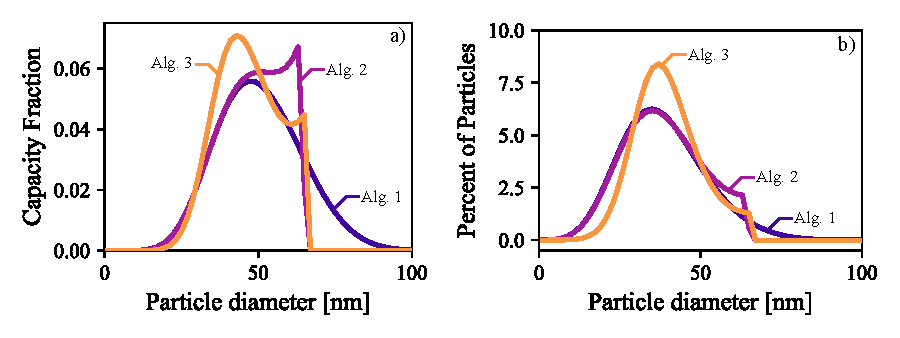
\includegraphics[scale=1]{figures/Sup_PSDs_combined.pdf}
    \caption{\textcolor{red}{ PSD snapshots from then end of the simulated discharge described in Archer and Lau.~\cite{bib:Verify}. Results presented as a fraction of \textbf{a)} total capacity and \textbf{b)} total number of particles. Algorithm 1 allows particles to diffuse into a normal distribution. Nucleation is continuous throughout the simulation so Algorithm 2 is only bounded by a leading bookmark causing particles to build up at the leading edge. Algorithm 3 employs the `moving	hopper' model and matches the distribution from Archer and Lau. }}
    \label{fig:Sup_PSDs}
\end{figure}

\begin{table}[h!]
  \centering
  \caption{Comparison of the performance of the three algorithms in replicating the the results from Lau and Archer\cite{bib:Verify}. Algorithm 3 is the baseline for the percent error calculation. The simulated discharge capacity in Lau and Archer was just above 2.5 mAh.}
  \label{Table}
  \begin{tabular}{lccc}
  \toprule[1pt]\midrule[0.3pt]
      Algorithm & Capacity [mAh] & Run Time [s] & Avg. Error [\%] \\
      \midrule
       1   & 2.505 & 0.449  & 176.7\\
       2 & 2.431 & 2.902 & 176.7\\
       3 & 2.500 & 0.769 & -- \\ 
       \midrule[0.3pt]\bottomrule[1pt]
  \end{tabular}

\end{table}
 
\textcolor{red}{The resulting PSDs for our three algorithms above are shown in Figure~\ref{fig:Sup_PSDs}, below, and the total discharge capacity, simulation time, and quantitative error calculations for each are provided in Table~\ref{Table}. The three algorithms give notably different PSD shapes. The `bookmark' approach from algorithm 2 (Figure~\ref{fig:Sup_PSDs}a) fared the worst, failing to match the overall discharge capacity and taking the longest time to run.  The distributions in Figure~\ref{fig:Sup_PSDs} are presented in terms of both capacity fraction (subfigure a) and percent of particles in each bin (subfigure b).  }

\textcolor{red}{Algorithm 3, the `moving hopper' model correctly predicts the PSD shape and discharge capacity from the reference publication,~\cite{bib:Verify} and takes only 320 ms longer than algorithm 1. This is a significant increase (71\%) relative to the Algorithm 1 simulation time. However, as additional model equations are added to track electrolyte chemistry, electric potential, and other  variables, the impact of adding one new equation at each physical location will have lower relative impact.}

\textcolor{red}{While algorithm 1 matches the overall  reference publication capacity, the differences in PSD will have increasing impact as simulations are used to predict extended cycling in realistic situations. For example, if the battery is not fully recharged (i.e., deposits not fully removed) before charging resumes, the particles at the low-diameter end of the PSD will erode, but the high-diameter portion of the PSD would remain. The shape of the PSD when discharge resumes will impact the available surface area for growth, the resulting degree of supersaturation, and the particle sizes that develop during discharge, impacting subsequent battery performance.}\\ 

\noindent(3) The normalization of the PSD and the meanings of the plotted axes are not always clearly specified in the figures; additional clarification would improve readability and reproducibility. \\ 

\noindent\textcolor{blue}{The focus of our analysis is on the shape of the PSD as it evolves with time. The nominal height is not a focus of comparison. The physical number of particles in each bin is not data point we compare between methods, so we chose to normalize the PSD. We used the total number of particles because it is a consistent baseline for all time steps.}\\ 

\noindent\textcolor{blue}{On page 3 we added a section to clarify the normalization and explain our reasoning:} \textcolor{red}{``The simulation inputs have the same order of magnitude as real parameters."}\textcolor{blue}{and on page 5 we clarified the meaning of the axes,}\textcolor{red}{ ``and the total number of particles remains constant for the remainder of the simulation. We normalized the y-axis data by dividing the number particles in each bin by the total number of particles deposited. Because the PSD shape is the point of emphasis, here, the actual particle concentrations are not of particular importance, and concentration differences between one algorithm and the next would only serve to distract from the salient features."}
\\

\noindent Overall, this work offers a valuable numerical-methods contribution to modeling deposition reactions in batteries, and I recommend acceptance after minor revision addressing the points above. \\ \\
\noindent\textcolor{blue}{We thank the reviewer for their helpful suggestions and kind comments.}\\ \\

\noindent \textbf{Reviewer: 2}  \\

\noindent Recommendation: This paper is not recommended because the material is not appropriate for the Journal of Physical Chemistry. \\

\noindent Comments: \\
Title: Particle Tracking Methods for Battery Precipitation Reactions
Authors: Trent Koberna, Steven C. DeCaluwe \\
The present work provides a theoretical work for modelling deposition reactions in battery chemistry. The authors present a comparison of several approaches to model the temporal evolution of particle size distribution of deposits on electrode surfaces. In its actual version the work can’t be published in the article section of the Journal of Physical Chemistry. \\

\noindent1.The authors present a purely theoretical model without any validation against alternative simulation approaches, theoretical predictions, or experimental data from the literature. As it stands, it is not possible to assess the validity of the proposed algorithms. \\

\noindent\textcolor{blue}{The thrust of the paper was intended to compare potential methodologies and to illustrate the pitfalls in using a finite difference approach. The parameters of the simulation: a singular, finite nucleation period and consistent growth rate for all particles should result in a PSD that is invariant once nucleation is complete. This known outcome was sufficient for us to determine that Algorithm 1 and 2 were inaccurate. However, you are absolutely correct that validation against an additional source would increase the value of the manuscript, by demonstrating the validity and utility of Algorithm 3. We added another section to the discussion on pages 9 and 10.} \\

\textcolor{red}{While the above results are intentionally technology agnostic so as to focus on the algorithmic components and the resulting inconsistency between model results and assumptions, it is worth exploring whether these inconsistencies meaningfully impact actual battery simulations. To test this, we implemented the Li-O$_2$ battery model descried in Lau and Archer~\cite{bib:Verify} and  replicated the particle size distribution shown in Figure 5b of that publication. The Archer and Lau model assumes a constant nucleation rate that remains active during the entire discharge process. This provides a different set of conditions, with technologically-relevant chemical rates, in which to evaluate the impact of the algorithms considered above.}    


\begin{figure}[h]
    \centering
    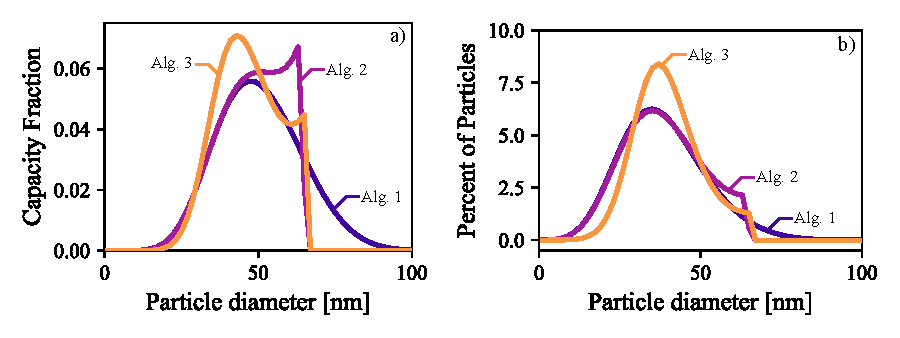
\includegraphics[scale=1]{figures/Sup_PSDs_combined.pdf}
    \caption{\textcolor{red}{ PSD snapshots from then end of the simulated discharge described in Archer and Lau.~\cite{bib:Verify}. Results presented as a fraction of \textbf{a)} total capacity and \textbf{b)} total number of particles. Algorithm 1 allows particles to diffuse into a normal distribution. Nucleation is continuous throughout the simulation so Algorithm 2 is only bounded by a leading bookmark causing particles to build up at the leading edge. Algorithm 3 employs the `moving	hopper' model and matches the distribution from Archer and Lau. }}
    \label{fig:Sup_PSDs}
\end{figure}

\begin{table}[h!]
  \centering
  \caption{Comparison of the performance of the three algorithms in replicating the the results from Lau and Archer\cite{bib:Verify}. Algorithm 3 is the baseline for the percent error calculation. The simulated discharge capacity in Lau and Archer was just above 2.5 mAh.}
  \label{Table}
  \begin{tabular}{lccc}
  \toprule[1pt]\midrule[0.3pt]
      Algorithm & Capacity [mAh] & Run Time [s] & Avg. Error [\%] \\
      \midrule
       1   & 2.505 & 0.449  & 176.7\\
       2 & 2.431 & 2.902 & 176.7\\
       3 & 2.500 & 0.769 & -- \\ 
       \midrule[0.3pt]\bottomrule[1pt]
  \end{tabular}

\end{table}
 
\textcolor{red}{The resulting PSDs for our three algorithms above are shown in Figure~\ref{fig:Sup_PSDs}, below, and the total discharge capacity, simulation time, and quantitative error calculations for each are provided in Table~\ref{Table}. The three algorithms give notably different PSD shapes. The `bookmark' approach from algorithm 2 (Figure~\ref{fig:Sup_PSDs}a) fared the worst, failing to match the overall discharge capacity and taking the longest time to run.  The distributions in Figure~\ref{fig:Sup_PSDs} are presented in terms of both capacity fraction (subfigure a) and percent of particles in each bin (subfigure b).  }

\textcolor{red}{Algorithm 3, the `moving hopper' model correctly predicts the PSD shape and discharge capacity from the reference publication,~\cite{bib:Verify} and takes only 320 ms longer than algorithm 1. This is a significant increase (71\%) relative to the Algorithm 1 simulation time. However, as additional model equations are added to track electrolyte chemistry, electric potential, and other  variables, the impact of adding one new equation at each physical location will have lower relative impact.}

\textcolor{red}{While algorithm 1 matches the overall  reference publication capacity, the differences in PSD will have increasing impact as simulations are used to predict extended cycling in realistic situations. For example, if the battery is not fully recharged (i.e., deposits not fully removed) before charging resumes, the particles at the low-diameter end of the PSD will erode, but the high-diameter portion of the PSD would remain. The shape of the PSD when discharge resumes will impact the available surface area for growth, the resulting degree of supersaturation, and the particle sizes that develop during discharge, impacting subsequent battery performance.} \\ \\

\noindent2.The authors claim that the model is applicable to a variety of deposition scenarios relevant to battery applications, particularly the solid electrolyte interphase (SEI). However, the description of the deposition reactions, as outlined between lines 23 and 42 on page 3, employs a two-step mechanism. This representation is overly simplistic and unsuitable for modeling SEI formation. During the early stages of decomposition reactions—typically occurring at the electrode-electrolyte interface and during initial cycling steps—small molecules accumulate and undergo polymerization/condensation reactions. This process results in the formation of a dense, porous, and amorphous phase, which is far more complex than the scenario described in the paper. \\

\noindent\textcolor{blue}{We have removed the section about SEI formation from page 1 of the article and expanded upon two battery chemistries with interfacial growth.} \\

    \begin{itemize}
        \item \textcolor{red}{\textit{Lithium-sulfur}: In lithium-sulfur batteries, polysulfide species dissolved in the liquid electrolyte are reduced during discharge, depositing and growing on the cathode surface as low-order polysulfide (e.g., Li$_2$S) precipitates. The capacity and rate capability are sensitive to the precipitate nucleation density~\cite{bib:Li-S_deposition,bib:Li-S_deposition_2,bib:Model_ex_8}.}
               
        \item \textcolor{red}{\textit{Lithium-air}: In lithium-air batteries, oxygen dissolves into the liquid electrolyte from a cathode flow channel are reduced during discharge, depositing and growing on the cathode surface as lithium oxide (Li$_2$O) and peroxide (Li$_2$O$_2$). The precipitate morphology plays a significant role in determining the overall cathode utilization and porous cathode transport properties during battery cycling, which significantly impact battery performance~\cite{bib:Li-O_deposition,bib:Li-air_deposition}.}
        
        \item \textcolor{red}{\sout{\textit{SEI formation}: The solid electrolyte interphase (SEI) is a multi-phase passivation layer on the anode surface, formed via deposition of insoluble electrolyte degradation products. The number, size, and distribution of individual phases determine the layer's ionic conductivity and long-term stability and are controlled by nucleation and growth phenomena~\cite{bib:SEI_deposition,bib:SEI_deposition_2,bib:SEI_deposition_3}.}}
    \end{itemize}

\noindent3. Several figures, particularly Figures 2 and 4, are superimposed, rendering the results difficult to review and interpret effectively. \\

\noindent\textcolor{blue}{The overlap of the figures was a result of reformatting of the article after submission.} \\

\noindent\textcolor{blue}{Again, we thank the reviewers for their attention and input. Their contributions have made this a stronger publication.} \\

\noindent\textcolor{blue}{The conclusion was expanded on pages 10 and 11 to further clarify the utility and impact of algorithm 3.} \\
\textcolor{red}{As heterogeneous nucleation and growth phenomena become increasingly important in a range of energy storage and conversion technologies, in batteries and beyond, attention to the particle size distribution tracking will require greater attention. In this study, initial attempts at tracking particle growth using standard spatial discretization methods resulted in flattening between bins that distorted the PSD. To solve this type of anomalous `particle diffusion' between discretized radial bins, we propose here a `moving hopper' model that controls which bin particles are deposited into instead of moving particles between bins. Once deposited, a particle remains in a given discretized bin/position within the solution vector; rather than moving particles to a different bin as they grow, this approach alters the average radius associated with the particles' current bin. The approach only requires two differential equations, at any given time--one rate for the bin where deposition occurs and one for the growth rate of the largest particle--supporting computational efficiency.}

\bibliographystyle{unsrt}
\bibliography{bibliography}
\end{document}
